\chapter{Amplificadores Realimentados}




\hspace{10pt} \textbf{Ejercicio 1 :} Se requiere insensibilizar la ganancia de un
amplificador realimentado ante cambios en la ganancia sin
realimentar \textbf{$a_o$}. La ganancia a lazo cerrado debe ser $A_f
= -200$. Además ésta no debe variar más del $1\%$ a pesar de las
variaciones de un $40\%$ en $a_o$. Determinar $a_o$ y $f$ y
verificar que $A_f$ es aproximadamente igual a $\frac{\displaystyle
	1}{\displaystyle f}$. Si se quiere también una tensión de salida
$V_o = 10V$, calcular los valores de las tensiones de entrada,
realimentada y de error correspondientes. Ver figura \ref{eje1}
\begin{figure}[h]
	\centering
	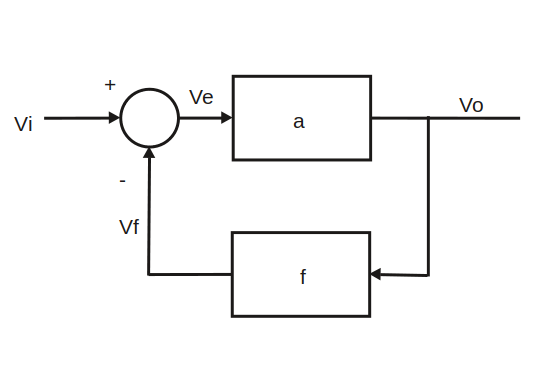
\includegraphics[width=0.6\linewidth]{figuras/real1.png}\\
	\caption{Ejercicio 1.}\label{eje1}
\end{figure}

\textbf{Ejercicio 2 :} La figura \ref{eje2} muestra la curva de
transferencia de un amplificador básico, la cual es evidentemente
alineal. Suponga $f = 0,1$, dibuje la nueva curva de transferencia
total y extraiga conclusiones.

\begin{figure}[h]
	\centering
	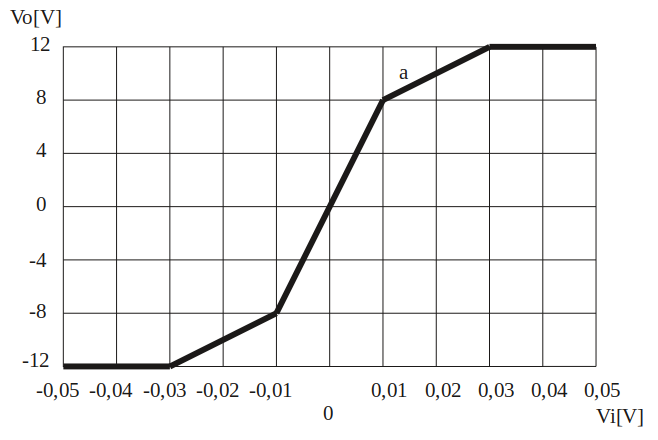
\includegraphics[width=0.6\linewidth]{figuras/real2.png}\\
	\caption{Ejercicio 2.}\label{eje2}
\end{figure}

\textbf{Ejercicio 3}: Se dispone de un amplificador con ganancia de
tensión $a_1=100$, por problemas de filtrado en la fuente de
alimentación aparece una tensión de ruido $v_r = 10mV$ en su
entrada, hallar la relación señal a ruido si la salida de señal útil
es $v_o=1V$. Realimentar el circuito agregando una etapa no ruidosa
a la entrada de ganancia $a_2=10000$, de modo que la ganancia del
circuito modificado sea igual a la ganancia $a_1$. Recalcule la
relación señal a ruido utilizando los mismos niveles de tensión en
la salida y de ruido en la etapa de salida, extraiga conclusiones.


\textbf{Ejercicio 4:} Determinar si la realimentación en los
circuitos de la figura \ref{eje4} es positiva o negativa.


\begin{figure}[h]
	\centering
	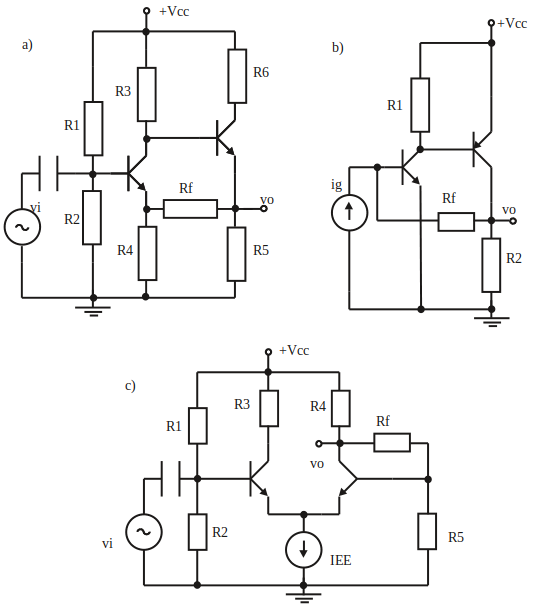
\includegraphics[width=0.6\linewidth]{figuras/real4.png}\\
	\caption{Ejercicio 4.}\label{eje4}
\end{figure}


\textbf{Ejercicio 5} : Suponiendo que el modelo del amplificador sin
realimentar es el mostrado en la figura \ref{eje5}, hallar:
$\frac{\displaystyle v_o}{\displaystyle v_i}$, $Z_i$ y $Z_o$ en los
casos a) y b).



\begin{figure}[h]
	\centering
	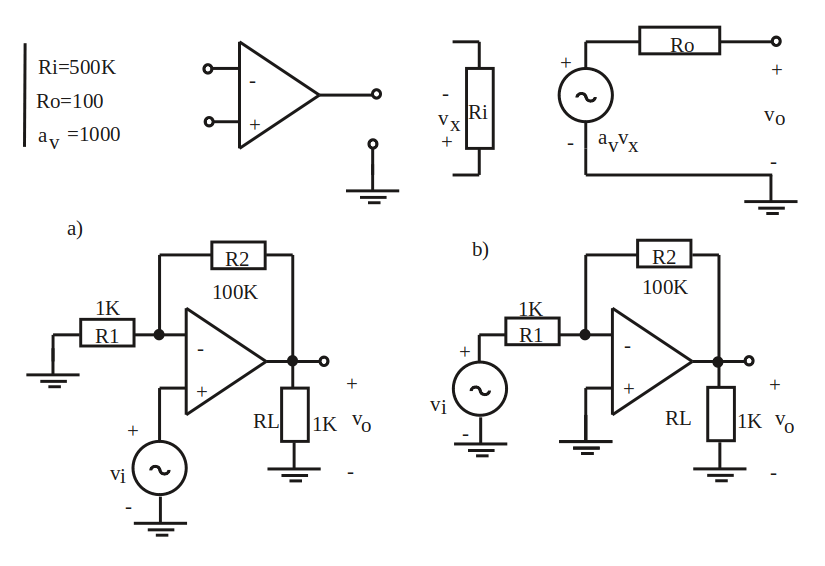
\includegraphics[width=0.6\linewidth]{figuras/real5.png}\\
	\caption{Ejercicio 5.}\label{eje5}
\end{figure}


\textbf{Ejercicio 6} : Se desea manejar una carga $R_L$  con un
amplificador de corriente de ganancia $A_i=-10$ , el amplificador
debe tender a comportarse como uno ideal. Para ello se cuenta con el
amplificador de corriente sin realimentar mostrado en la figura
\ref{eje6}, siendo el generador de entrada el generador real de
corriente $i_G$. Realimentar el circuito con una red resistiva
apropiada para lograr el objetivo, hallar los valores de impedancias
de entrada y salida.

\begin{figure}[h]
	\centering
	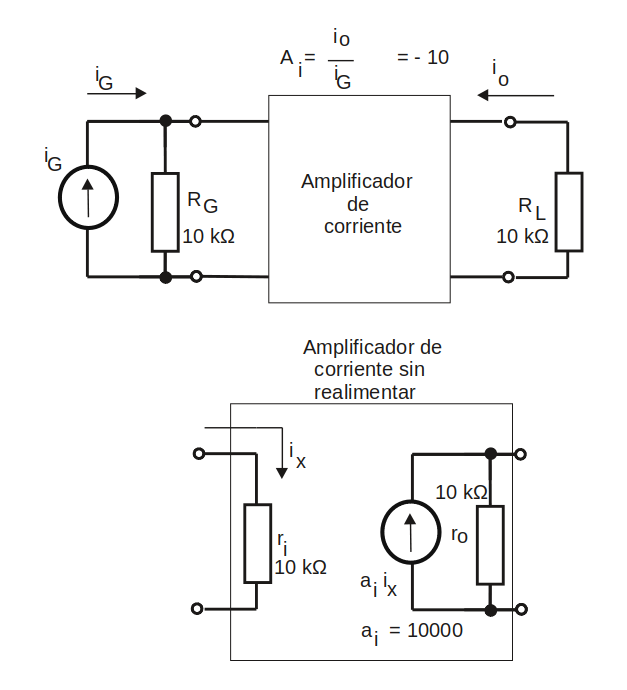
\includegraphics[width=0.6\linewidth]{figuras/real6.png}\\
	\caption{Ejercicio 6.}\label{eje6}
\end{figure}

\textbf{Ejercicio 7} : Demostrar, por el método de cuadripolos, lo
expresado en el circuito de la figura \ref{eje7}.

\begin{figure}[h]
	\centering
	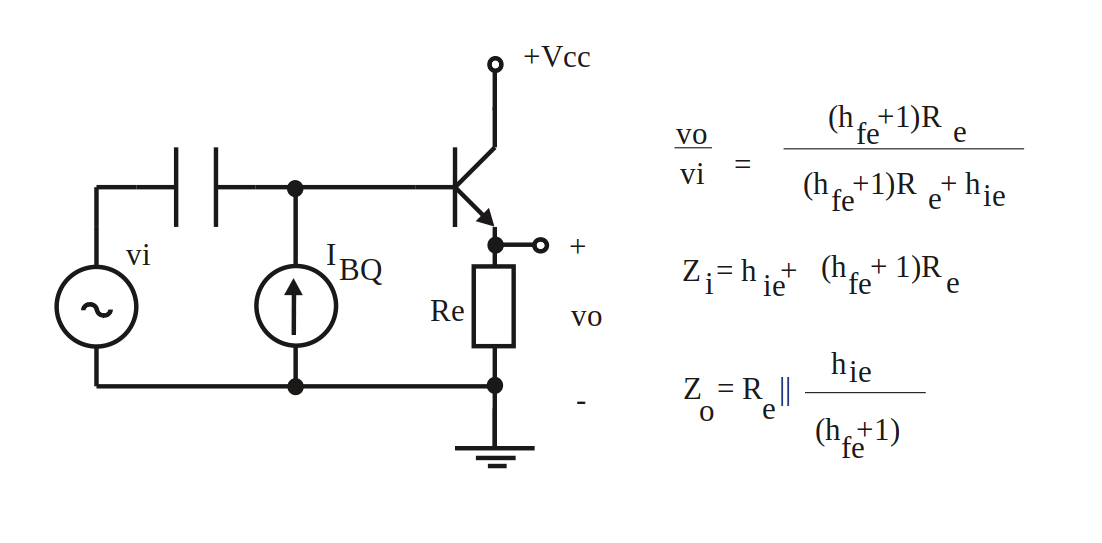
\includegraphics[width=0.6\linewidth]{figuras/real7.png}\\
	\caption{Ejercicio 7.}\label{eje7}
\end{figure}


\textbf{Ejercicio 8} : Suponiendo que el circuito de la figura
\ref{eje8} es el equivalente de corriente alterna de un circuito
realimentado correctamente polarizado: hallar $T_o$ y comparar
cualitativamente cómo se comporta la impedancia de entrada respecto
al caso de lazo abierto.

\begin{figure}[h]
	\centering
	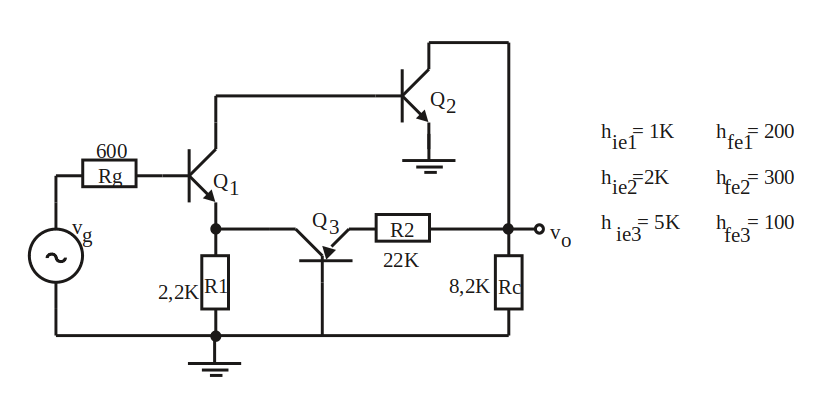
\includegraphics[width=0.8\linewidth]{figuras/real8.png}\\
	\caption{Ejercicio 8.}\label{eje8}
\end{figure}

\textbf{Ejercicio 9} : En el circuito de la figura \ref{eje9},
calcular la ganancia de tensión por cuadripolos y verificar su
resultado mediante otro método (mallas o simulación). Sacar
conclusiones.

\begin{figure}[h]
	\centering
	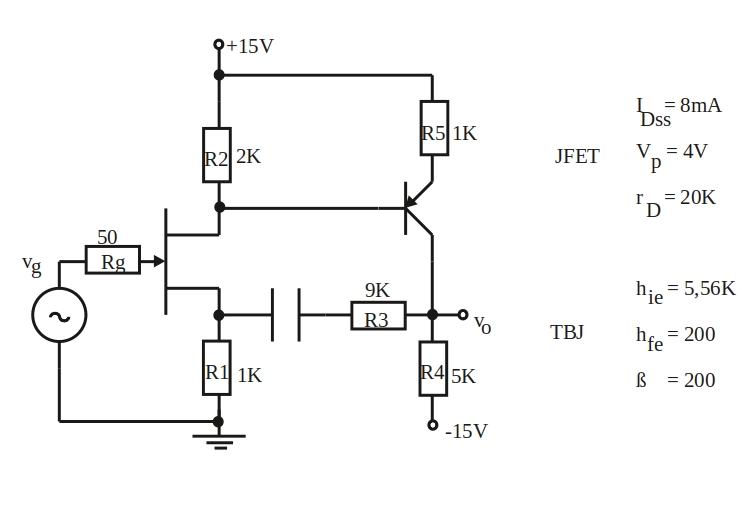
\includegraphics[width=0.8\linewidth]{figuras/real9.png}\\
	\caption{Ejercicio 9.}\label{eje9}
\end{figure}


\textbf{Ejercicio 10} : En el circuito de la figura \ref{eje10},
obtener $\frac{\displaystyle v_o}{\displaystyle v_i}$, $Z_i$ y
$Z_o$.

\begin{figure}[h]
	\centering
	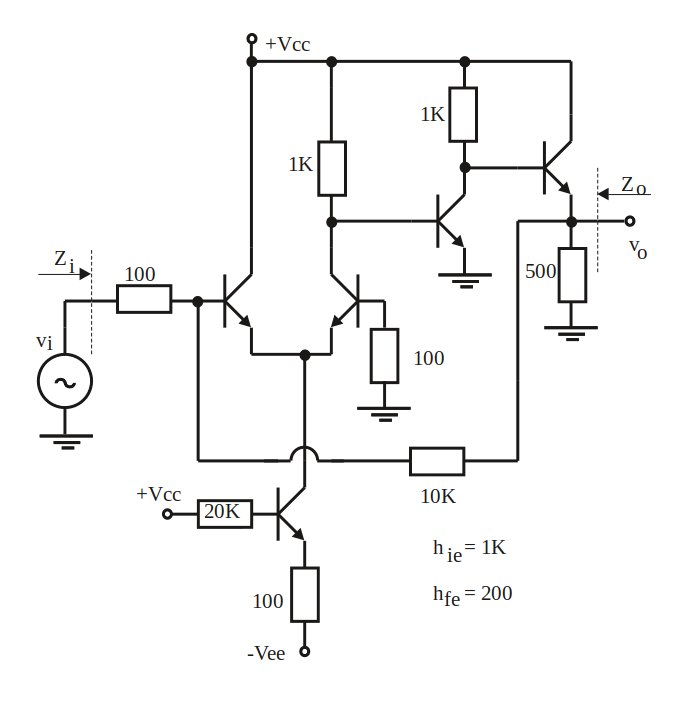
\includegraphics[width=0.8\linewidth]{figuras/real10.png}\\
	\caption{Ejercicio 10.}\label{eje10}
\end{figure}

\textbf{Ejercicio 11} : En el circuito de la figura \ref{eje11},
hallar, a) $R_x$ si $Z_i=55 \Omega$ ,  b) $\frac{\displaystyle
	v_o}{\displaystyle v_i}$ y c) $Z_o$.

\begin{figure}[h]
	\centering
	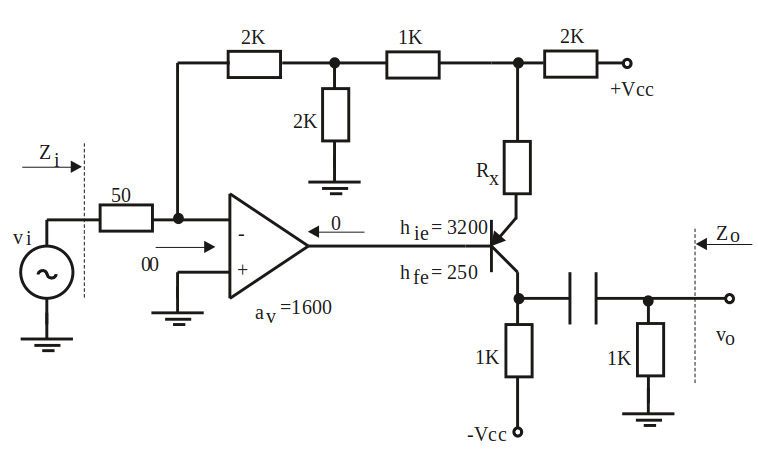
\includegraphics[width=0.8\linewidth]{figuras/real11.png}\\
	\caption{Ejercicio 11.}\label{eje11}
\end{figure}

\textbf{Ejercicio 12} : En el circuito de la figura \ref{eje12}
determinar la polaridad del amplificador de tensión para que la
realimentación sea negativa. Efectuando mediciones se obtuvo,
además, que $|v_o|=1V$ y $|v_i|=100mV$. Calcular $R_f$ y $Z_o$.


\begin{figure}[h]
	\centering
	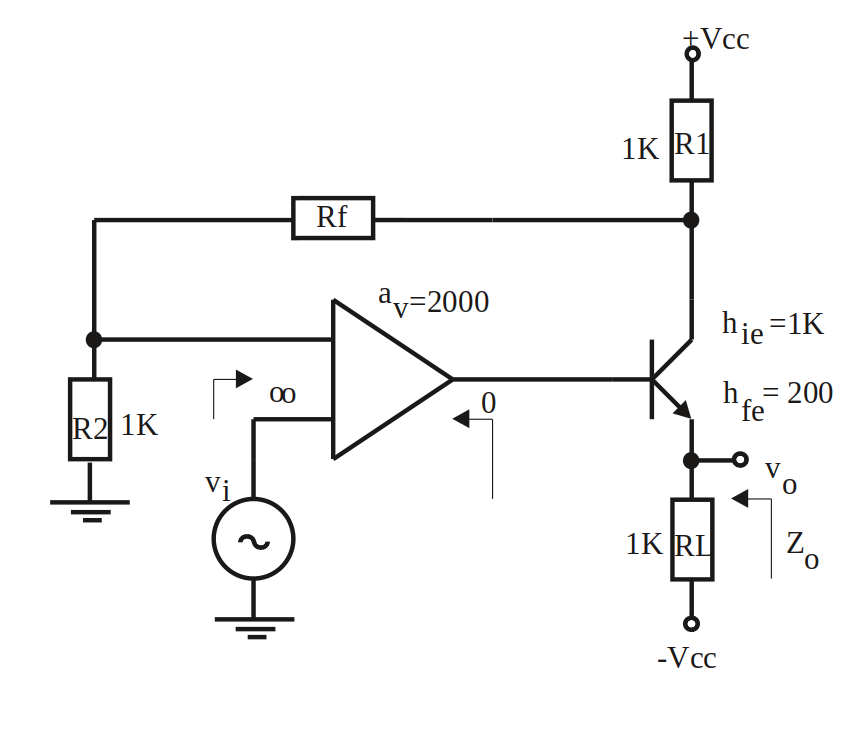
\includegraphics[width=0.8\linewidth]{figuras/real12.png}\\
	\caption{Ejercicio 12.}\label{eje12}
\end{figure}

\textbf{Ejercicio 13} : En el circuito de la figura \ref{eje13},
obtener: a) la ganancia $\frac{\displaystyle v_{o1}}{\displaystyle
	v_g}$, la impedancia de entrada que ve el generador $v_g$ y la
impedancia de salida $Z_{o1}$ ; b) la ganancia $\frac{\displaystyle
	v_{o2}}{\displaystyle v_g}$, la impedancia de entrada que ve el
generador $v_g$ y la impedancia de salida $Z_{o2}$ , c) comparar
ambos resultados y sacar conclusiones.

\begin{figure}[h]
	\centering
	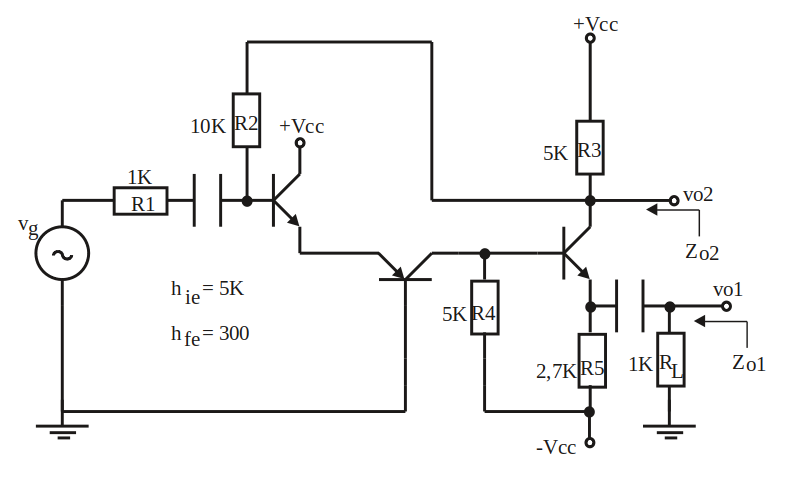
\includegraphics[width=0.8\linewidth]{figuras/real13.png}\\
	\caption{Ejercicio 13.}\label{eje13}
\end{figure}


